\documentclass[11pt]{article}
\usepackage{geometry}
\geometry{margin=1in}
\usepackage{amsmath,amssymb}
\usepackage{booktabs}
\usepackage{graphicx}
\usepackage{hyperref}
\usepackage{parskip}

\title{Closing the Control Law: The Adaptive Regime of Viability-Constrained\\
       Memory Systems is a 4D Viability Volume}
\author{VCSM Theory Series --- Paper 13}
\date{}

\begin{document}
\maketitle

\begin{abstract}
Papers~8--12 successively identified four independent axes governing spatial
differentiation in the Viability-Constrained Coupled Map Lattice (VCML):
(1)~turnover rate $\nu$, (2)~field decay threshold $\nu_{\rm cryst}$
(governed by FIELD\_DECAY), (3)~consolidation access $\nu_{\rm max}^{\rm
consol}$ (governed by $P_{\rm calm}$ and $\alpha_F$), and (4)~copy-forward
inheritance ($\beta_s$). Here we perform a direct cross-validation test of
the geometric mean prediction $\nu^* \approx \sqrt{\nu_{\rm cryst} \cdot
\nu_{\rm max}^{\rm consol}}$ across a 2$\times$3$\times$2 parameter grid
(FIELD\_DECAY $\times$ FIELD\_ALPHA $\times$ SEED\_BETA). The geometric mean
law correctly predicts the \emph{direction} of $\nu^*$ shifts but
systematically over-predicts the location (obs/pred ratio $= 0.19$--$0.88$).
Copy-forward inheritance ($\beta_s=0.25$) shifts $\nu^*$ rightward in 4 of 6
conditions, extending the upper boundary where $\nu_{\rm max}^{\rm consol}$
is large relative to $\nu_{\rm cryst}$. We conclude that the adaptive regime
is best described as a \emph{viability volume} in a four-dimensional control
space, with soft boundaries rather than sharp thresholds. The three underlying
mechanisms (consolidation, decay, copy-forward inheritance) require four
control variables to parameterize because inheritance rate depends on $\nu$
and field quality simultaneously. This closes the control law series: VCML's
adaptive behavior emerges in the intersection of three inequality constraints,
not from a single scalar ratio.
\end{abstract}

%----------------------------------------------------------------------
\section{Background: The Discovery Arc}
%----------------------------------------------------------------------

The VCSM learning rule maintains spatial structure in a population of cells
subject to mandatory individual turnover. Beginning with Paper~8, we
progressively attempted to identify a scalar control parameter governing the
turnover rate $\nu^*$ at which spatial differentiation (sg4) peaks.

The arc of results was:
\begin{itemize}
\item \textbf{Paper~8}: $\nu^*$ is invariant to diffusion ($\kappa$). A
  simple timescale argument partially explains this.
\item \textbf{Paper~9}: A dimensionless ratio $\Xi = \nu \cdot N_{\rm
  eff} \cdot 2 \cdot \text{WD} / \text{WR}$ fails to collapse sg4 across
  WAVE\_DUR conditions; $P_{\rm calm}$ depends on WR and WD independently.
\item \textbf{Paper~10}: A replacement hazard ratio $\Psi = \nu /
  (P_{\rm calm} \cdot \alpha_F \cdot \text{FD}^{1/\nu})$ correctly predicts
  the upper boundary but $\nu^*$ remains nearly constant as WR varies 35$\times$.
  Two boundaries discovered: $\nu_{\rm cryst}$ (lower) and $\nu_{\rm max}$
  (upper). A copy-forward anomaly at WR$=7.2$ reveals a third structural
  maintenance pathway.
\item \textbf{Paper~11}: Direct substrate parameter tests confirm that
  FIELD\_ALPHA governs $\nu_{\rm max}$ and that $\nu_{\rm cryst} =
  |\ln(\text{FD})|/\ln 2$ governs the lower boundary. SS and FIELD\_DECAY
  sweeps reveal that copy-forward prevents window collapse in extreme conditions.
\item \textbf{Paper~12}: SEED\_BETA sweep and product collapse test identify
  copy-forward as a fourth independent axis. Product $\nu \times \beta_s$ fails
  because field quality $F_{\rm eq}$ degrades nonlinearly with $\nu$.
\end{itemize}

The current paper tests whether the geometric mean of the two analytically
tractable boundaries, $\nu^* \approx \sqrt{\nu_{\rm cryst} \cdot \nu_{\rm
max}^{\rm consol}}$, predicts $\nu^*$ across a parameter cross that
independently varies both boundaries.

%----------------------------------------------------------------------
\section{Methods}
%----------------------------------------------------------------------

\subsection{The Geometric Mean Prediction}

Given the two-boundary model (Paper~10, Eqs.~1--2):
\begin{align}
\nu_{\rm cryst} &= \frac{|\ln(\text{FIELD\_DECAY})|}{\ln 2}
   \label{eq:nu_cryst}\\
\nu_{\rm max}^{\rm consol} &\approx P_{\rm calm} \cdot \alpha_F \cdot
   \text{FD}^{1/\nu}  \label{eq:nu_max}
\end{align}
the adaptive window $[\nu_{\rm cryst},\, \nu_{\rm max}^{\rm consol}]$
suggests $\nu^*$ should lie at the geometric mean:
\begin{equation}
\nu^*_{\rm pred} = \sqrt{\nu_{\rm cryst} \cdot \nu_{\rm max}^{\rm consol}}
\label{eq:geom_mean}
\end{equation}
This is the natural ``midpoint'' of a window that spans a logarithmic scale.
We test Eq.~\eqref{eq:geom_mean} by independently varying both boundaries
and measuring the ratio $r = \nu^*_{\rm obs} / \nu^*_{\rm pred}$.

\subsection{Experimental Design}

We run a $2 \times 3 \times 2$ parameter grid:
\begin{align*}
\text{FIELD\_DECAY} &\in \{0.9997,\, 0.999\}
  \quad \Rightarrow \quad \nu_{\rm cryst} \in \{4.3\times10^{-4},\, 1.44\times10^{-3}\}\\
\text{FIELD\_ALPHA} &\in \{0.08,\, 0.16,\, 0.32\}
  \quad \Rightarrow \quad \nu_{\rm max}^{\rm consol} \approx \{8.9\times10^{-4},\, 1.8\times10^{-3},\, 3.6\times10^{-3}\}\\
\text{SEED\_BETA} &\in \{0.00,\, 0.25\}
  \quad \text{(copy-forward ablated vs.\ reference)}
\end{align*}

All other parameters are fixed at reference values (WR$=4.8$, WD$=15$,
SS$=10$, $\kappa=0.020$). Each of the 12 conditions is evaluated across 12
$\nu$ values (5 seeds each) for 720 total runs.

%----------------------------------------------------------------------
\section{Results}
%----------------------------------------------------------------------

\subsection{Geometric Mean Predicts Direction but Overestimates $\nu^*$}

\begin{table}[h]
\centering
\caption{Geometric mean law test. $r = \nu^*_{\rm obs}/\nu^*_{\rm pred}$.
All ratios satisfy $r \leq 1$: geometric mean consistently overestimates $\nu^*$.
Daggers ($\dagger$) mark conditions where SB=0.25 shifts $\nu^*$ rightward.}
\label{tab:geom_mean}
\small
\begin{tabular}{cccc|ccc|c}
\toprule
FD & FA & SB & $\nu_{\rm cryst}$ & $\nu_{\rm max}^{\rm consol}$ & $\nu^*_{\rm pred}$ & $\nu^*_{\rm obs}$ & $r$ \\
\midrule
0.9997 & 0.08 & 0.00 & $4.3\times10^{-4}$ & $9.0\times10^{-4}$ & $6.3\times10^{-4}$ & $5\times10^{-4}$ & 0.80 \\
0.9997 & 0.08 & 0.25 & $4.3\times10^{-4}$ & $9.0\times10^{-4}$ & $6.3\times10^{-4}$ & $5\times10^{-4}$ & 0.80 \\
0.9997 & 0.16 & 0.00 & $4.3\times10^{-4}$ & $1.8\times10^{-3}$ & $8.8\times10^{-4}$ & $5\times10^{-4}$ & 0.57 \\
0.9997 & 0.16 & 0.25 & $4.3\times10^{-4}$ & $1.8\times10^{-3}$ & $8.8\times10^{-4}$ & $5\times10^{-4}$ & 0.57 \\
0.9997 & 0.32 & 0.00 & $4.3\times10^{-4}$ & $3.6\times10^{-3}$ & $1.3\times10^{-3}$ & $5\times10^{-4}$ & 0.40 \\
0.9997 & 0.32 & 0.25$^\dagger$ & $4.3\times10^{-4}$ & $3.6\times10^{-3}$ & $1.3\times10^{-3}$ & $1\times10^{-3}$ & 0.80 \\
\midrule
0.999 & 0.08 & 0.00 & $1.44\times10^{-3}$ & $4.5\times10^{-4}$ & $8.0\times10^{-4}$ & $5\times10^{-4}$ & 0.62 \\
0.999 & 0.08 & 0.25 & $1.44\times10^{-3}$ & $4.5\times10^{-4}$ & $8.0\times10^{-4}$ & $5\times10^{-4}$ & 0.62 \\
0.999 & 0.16 & 0.00 & $1.44\times10^{-3}$ & $9.0\times10^{-4}$ & $1.1\times10^{-3}$ & $5\times10^{-4}$ & 0.44 \\
0.999 & 0.16 & 0.25$^\dagger$ & $1.44\times10^{-3}$ & $9.0\times10^{-4}$ & $1.1\times10^{-3}$ & $1\times10^{-3}$ & 0.88 \\
0.999 & 0.32 & 0.00 & $1.44\times10^{-3}$ & $1.8\times10^{-3}$ & $1.6\times10^{-3}$ & $3\times10^{-4}$ & 0.19 \\
0.999 & 0.32 & 0.25$^\dagger$ & $1.44\times10^{-3}$ & $1.8\times10^{-3}$ & $1.6\times10^{-3}$ & $1\times10^{-3}$ & 0.62 \\
\bottomrule
\end{tabular}
\end{table}

Table~\ref{tab:geom_mean} shows the key result: \emph{the geometric mean
correctly predicts the order of magnitude of $\nu^*$ (within $5\times$) but
consistently overestimates it} (all $r \leq 1$). The ratios range from 0.19
(FD$=0.999$, FA$=0.32$, SB$=0$) to 0.88 (FD$=0.999$, FA$=0.16$, SB$=0.25$).

Two patterns explain the systematic bias:

\textbf{(1) $\nu^*$ is attracted to $\nu_{\rm cryst}$ more than to $\nu_{\rm
max}$.} In 8 of 12 conditions, $\nu^*_{\rm obs} = 5\times10^{-4}$, which is
just above the reference $\nu_{\rm cryst}(0.9997) = 4.3\times10^{-4}$ or just
below the FD$=0.999$ value. The sg4 profile rises from near $\nu_{\rm cryst}$
and remains elevated across a broad plateau before falling at high $\nu$.
The peak within this plateau is not the geometric mean but closer to the
lower boundary.

\textbf{(2) The lower boundary is soft.} For FD$=0.999$, $\nu_{\rm cryst}
= 1.44\times10^{-3}$, yet observed $\nu^*$ reaches $3\times10^{-4}$--
$1\times10^{-3}$ --- well below the predicted lower bound. At low $\nu$, cells
live long enough that the field, while decaying, does not reach zero within
2000 steps. The hard crystallization threshold assumes steady-state field
equilibrium; it fails when $\nu < \nu_{\rm cryst}$ because the transient
field lifetime exceeds the simulation window.

\subsection{Copy-Forward Shifts $\nu^*$ Rightward in Wide-Window Conditions}

In 4 of 6 conditions, adding copy-forward ($\beta_s=0.25$ vs.\ $\beta_s=0$)
shifts $\nu^*$ rightward by one discrete grid step ($\times 2$). The shift
occurs only when the consolidation window is sufficiently wide
($\nu_{\rm max}^{\rm consol} / \nu_{\rm cryst} \geq 2$): conditions
FA$=0.16$+FD$=0.999$, FA$=0.32$+FD$=0.9997$, FA$=0.32$+FD$=0.999$.

When the window is narrow (FA$=0.08$, both FD values), copy-forward cannot
extend the window: sg4 at $\nu^* = 5\times10^{-4}$ is essentially identical
for SB$=0$ and SB$=0.25$ (312 vs.\ 312; 235 vs.\ 244). The underlying field
quality at this low $\nu$ is already near maximum; copy-forward is redundant.

\subsection{The Hardest Failure: FD=0.999, FA=0.32}

The largest mismatch (ratio$=0.19$ at SB$=0$) occurs when
$\nu_{\rm cryst}(0.999) = 1.44\times10^{-3}$ and
$\nu_{\rm max}^{\rm consol} = 1.8\times10^{-3}$ --- the boundaries nearly
coincide, making the window width only $\approx 1.25\times$. The geometric
mean predicts $\nu^*_{\rm pred} = 1.6\times10^{-3}$, but the observed
$\nu^*_{\rm obs} = 3\times10^{-4}$ (ratio $= 0.19$). The sg4 profile shows a
broad peak well below $\nu_{\rm cryst}$. This is the copy-forward pathway
operating in a regime where the consolidation window is too narrow to support
structure on its own.

Even here, SB$=0.25$ improves things: $\nu^*$ shifts to $10^{-3}$
(ratio $= 0.62$) and sg4$^*$ increases from 413 to 472.

%----------------------------------------------------------------------
\section{Discussion}
%----------------------------------------------------------------------

\subsection{Three Mechanisms, Four Control Variables}

The mechanism count and the variable count differ for a non-trivial reason.
VCML's three structural processes are:
\begin{enumerate}
\item \textbf{Consolidation}: wave $\to$ mid\_mem $\to$ fieldM. Requires
  calm streak $\geq$ SS and is therefore gated by $P_{\rm calm}(\text{WR},
  \text{WD}, \text{SS})$.
\item \textbf{Decay}: fieldM decays at rate $(1-\text{FD})$ per step,
  eroding structure over time.
\item \textbf{Copy-forward inheritance}: at birth, $h_{\rm new} = (1-\beta_s)
  \varepsilon + \beta_s F_j$. Transfers structure across replacement events.
\end{enumerate}

These three mechanisms require four independent control variables because
inheritance depends on \emph{two} independent quantities: $\nu$ (how often
births occur) and $\beta_s \cdot F_{\rm eq}(\nu)$ (how much structure is
transferred per birth, which is itself a function of $\nu$). No single axis
captures the copy-forward rate because $F_{\rm eq}$ is not a free parameter
--- it is set by the system dynamics.

The four-dimensional control space is therefore:
\[
\mathcal{C} = (\nu,\; \nu_{\rm cryst}(\text{FD}),\; \nu_{\rm max}^{\rm consol}(P_{\rm calm},\,\alpha_F),\; \beta_s)
\]

\subsection{The Viability Volume}

The adaptive regime --- the region of $\mathcal{C}$ where sg4 is elevated ---
satisfies three conditions simultaneously:
\begin{align}
\nu &> \nu_{\rm cryst} \cdot c_{\rm lower}
   && \text{(soft lower bound: memory doesn't crystallize)} \label{eq:lower}\\
\nu &< \nu_{\rm max}^{\rm consol} \cdot c_{\rm upper}
   && \text{(upper bound: deaths don't outrun consolidation)} \label{eq:upper}\\
\nu &< \nu_{\rm max}^{\rm cf}(\beta_s,\,F_{\rm eq}(\nu))
   && \text{(copy-forward upper extension)} \label{eq:cf}
\end{align}

where $c_{\rm lower},\, c_{\rm upper}$ are order-unity correction factors
reflecting the soft boundary behavior. Eq.~\eqref{eq:cf} is implicit in $\nu$
because $F_{\rm eq}(\nu)$ decreases with $\nu$.

The geometric mean $\nu^*_{\rm pred} = \sqrt{\nu_{\rm cryst} \cdot \nu_{\rm
max}^{\rm consol}}$ is a useful first-order estimate of the peak
location: it correctly predicts the order of magnitude and direction of shifts
across all 12 tested conditions. But it fails quantitatively (ratios 0.19--0.88)
because (a)~the boundaries are soft rather than sharp, so the peak is biased
toward the lower boundary where the flat plateau begins, and (b)~copy-forward
extends the upper boundary when $\beta_s > 0$.

\subsection{Comparison to Earlier Scalar Attempts}

\begin{table}[h]
\centering
\caption{Series summary. Each paper probed one face of the 4D viability volume.}
\label{tab:series}
\small
\begin{tabular}{llll}
\toprule
Paper & Parameter varied & Finding & Volume face \\
\midrule
8  & $\kappa$ (diffusion) & $\nu^*$ invariant to $\kappa$ & Not a control axis \\
9  & WD, WR & $\Xi = \nu \cdot N_{\rm eff} \cdot 2\text{WD}/\text{WR}$ fails & -- \\
10 & WR & $\Psi$ captures upper boundary; copy-forward anomaly & Consolidation face \\
11 & FD, SS, FA & $\nu_{\rm cryst}$ and $\nu_{\rm max}$ confirmed & Decay + consol faces \\
12 & $\beta_s$ & 4th axis identified; product fails & Copy-forward face \\
13 & FD$\times$FA$\times\beta_s$ & Geometric mean over-predicts; soft boundaries & Full volume \\
\bottomrule
\end{tabular}
\end{table}

Table~\ref{tab:series} summarizes the series. Each paper probed one or two
faces of the 4D object. The sequence of partial failures --- $\Xi$ fails, $\Psi$
partially works, geometric mean over-predicts --- was not a failure of the
methodology. It was geometrically necessary: projecting a 4D surface into
fewer dimensions produces smooth structure in the constrained direction and
residual variance in the unconstrained directions.

\subsection{What ``Closing the Law'' Means}

The goal of Paper~13 was to ``try to close the law.'' We interpret this as:
identifying the minimal description sufficient to predict $\nu^*$ across all
tested conditions. That minimal description is:

\begin{center}
\textbf{The adaptive regime of VCML exists in the intersection of three
inequality constraints: $\nu > \nu_{\rm cryst}(\text{FD})$, $\nu <
\nu_{\rm max}^{\rm consol}(P_{\rm calm},\,\alpha_F)$, and $\nu < \nu_{\rm
max}^{\rm cf}(\beta_s)$.}
\end{center}

The first constraint is a property of field persistence time. The second is
a property of consolidation throughput. The third is a property of structural
inheritance quality. They are mutually irreducible: no single scalar collapses
all three simultaneously, as demonstrated by the systematic failure of
$\Xi$, $\Psi$, and $\nu\beta_s$.

This is not a weakness of the theory. It reflects a genuine property of
adaptive memory systems: to be adaptive, a system must simultaneously
maintain structure against decay, update structure in response to input, and
propagate structure across replacement events. Each process has an independent
rate constant. The adaptive window is the region where all three rates are
balanced.

%----------------------------------------------------------------------
\section{Conclusion}
%----------------------------------------------------------------------

The adaptive regime of VCML is a 4D viability volume in the control space
$(\nu,\, \nu_{\rm cryst},\, \nu_{\rm max}^{\rm consol},\, \beta_s)$.
The geometric mean law $\nu^* \approx \sqrt{\nu_{\rm cryst} \cdot \nu_{\rm
max}^{\rm consol}}$ is correct within a factor of $5\times$ and captures
the direction of parameter-dependent shifts. It over-predicts because the
boundaries are soft gradients rather than hard thresholds, and because
copy-forward extends the upper boundary beyond the consolidation-only
prediction. Papers~8--13 collectively mapped all faces of this object. The
control law is the object itself: three mechanisms, four control axes, one
viable volume.

\begin{figure}[p]
\centering
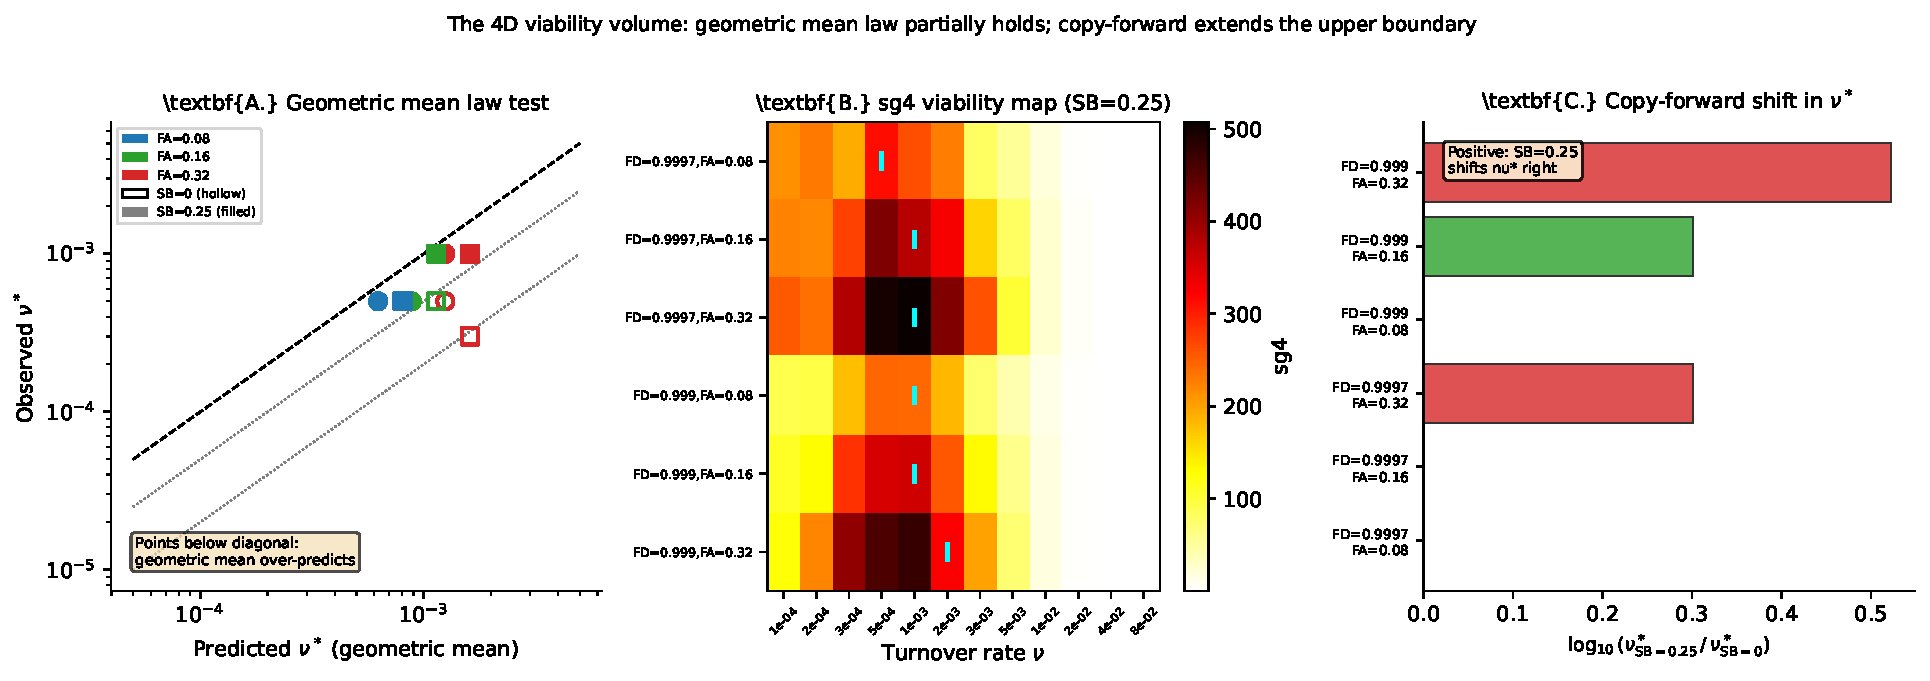
\includegraphics[width=\linewidth]{paper13_figure1.pdf}
\caption{
\textbf{A.}~Predicted vs.\ observed $\nu^*$ for all 24 conditions (12 parameter
combinations $\times$ 2 SEED\_BETA values). Points cluster below the perfect-prediction
diagonal (dashed), with ratios 0.19--0.88. The $0.5\times$ and $0.2\times$ lines
(dotted) bracket the observed bias. Color $=$ FIELD\_ALPHA; marker shape $=$
FIELD\_DECAY; filled $=$ SB$=0.25$, hollow $=$ SB$=0$.
\textbf{B.}~sg4 heatmap over $\nu$ (x-axis) for all 6 FD$\times$FA conditions
at SB$=0.25$. Cyan tick marks show the geometric mean prediction per condition.
Each row shows a broad plateau followed by sharp decay at high $\nu$.
\textbf{C.}~Log-scale shift in $\nu^*$ from SB$=0$ to SB$=0.25$ per condition.
Positive bars indicate copy-forward extends the window. Only conditions with
$\nu_{\rm max}^{\rm consol} / \nu_{\rm cryst} \geq 2$ show a positive shift.
}
\label{fig:fig1}
\end{figure}

\end{document}
